\documentclass{standalone}

\usepackage{tikz}
\usetikzlibrary{decorations.pathreplacing,calligraphy}

\begin{document}
	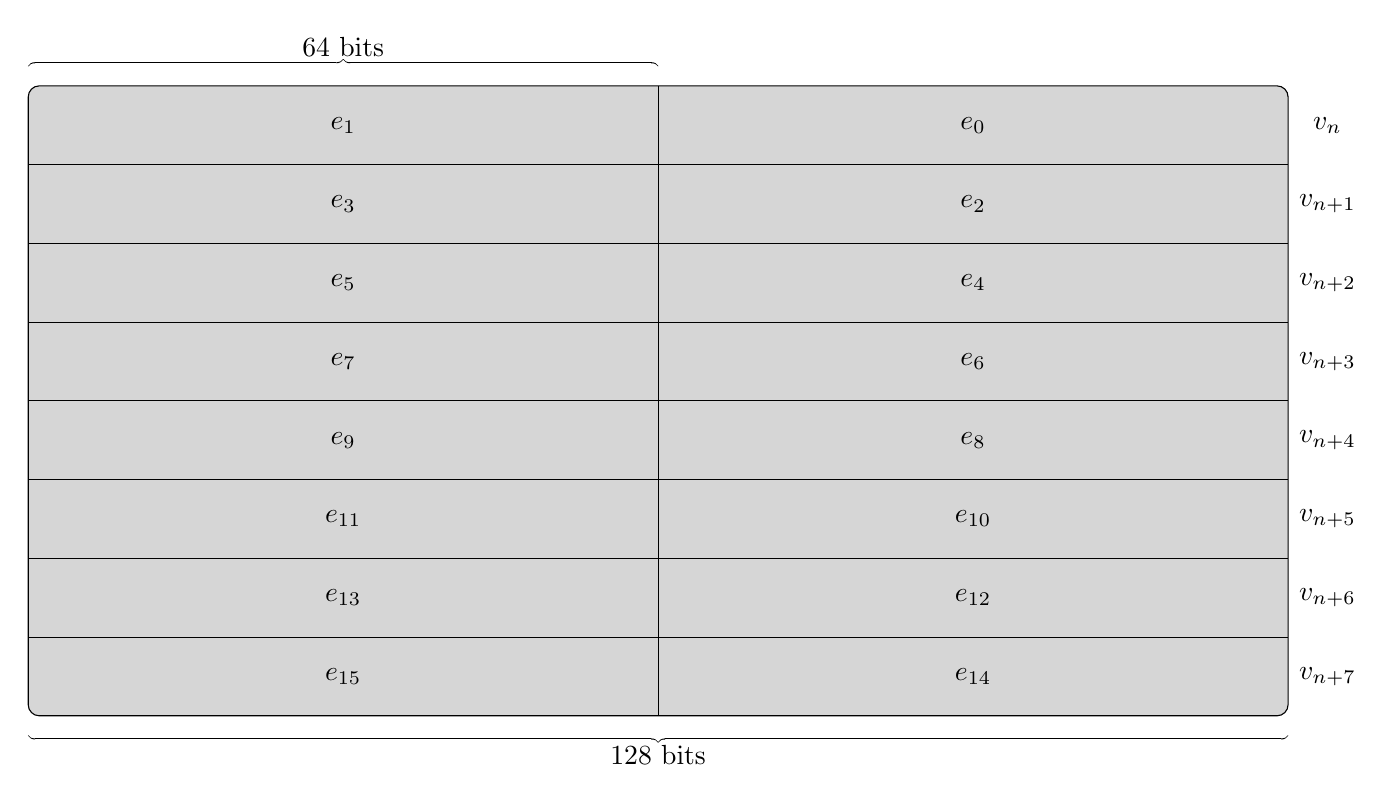
\begin{tikzpicture}
		\draw[fill=gray!32, rounded corners] (0, 0) rectangle (16, 8);
		\draw (8, 0) -- (8, 8);
		\draw (0, 1) -- (16, 1);
		\draw (0, 2) -- (16, 2);
		\draw (0, 3) -- (16, 3);
		\draw (0, 4) -- (16, 4);
		\draw (0, 5) -- (16, 5);
		\draw (0, 6) -- (16, 6);
		\draw (0, 7) -- (16, 7);
		
		\node at (4, 7.5) {$e_{1}$};
		\node at (12, 7.5) {$e_{0}$};
		\node at (4, 6.5) {$e_{3}$};
		\node at (12, 6.5) {$e_{2}$};
		\node at (4, 5.5) {$e_{5}$};
		\node at (12, 5.5) {$e_{4}$};
		\node at (4, 4.5) {$e_{7}$};
		\node at (12, 4.5) {$e_{6}$};
		
		\node at (4, 3.5) {$e_{9}$};
		\node at (12, 3.5) {$e_{8}$};
		\node at (4, 2.5) {$e_{11}$};
		\node at (12, 2.5) {$e_{10}$};
		\node at (4, 1.5) {$e_{13}$};
		\node at (12, 1.5) {$e_{12}$};
		\node at (4, 0.5) {$e_{15}$};
		\node at (12, 0.5) {$e_{14}$};
		
		\draw [decorate, decoration = {calligraphic brace}] (0, 8.25) --  (8, 8.25);
		\draw [decorate, decoration = {calligraphic brace, mirror}] (0, -0.25) --  (16, -0.25); 
		
		\node at (4, 8.5) {64 bits};
		\node at (8, -0.5) {128 bits};
		
		\node at (16.5, 7.5) {$v_{n}$};
		\node at (16.5, 6.5) {$v_{n+1}$};
		\node at (16.5, 5.5) {$v_{n+2}$};
		\node at (16.5, 4.5) {$v_{n+3}$};
		\node at (16.5, 3.5) {$v_{n+4}$};
		\node at (16.5, 2.5) {$v_{n+5}$};
		\node at (16.5, 1.5) {$v_{n+6}$};
		\node at (16.5, 0.5) {$v_{n+7}$};
	\end{tikzpicture}
\end{document}t